\subsection{\label{subsecEventSelection}Event selection and classification}

The data were collected using a minimum-bias trigger requiring a hit either in the A or C side of the V0 (denoted in what follows as V0A or V0C, respectively) or in the SPD, in coincidence with the arrival of proton bunches from both directions. Contamination from beam-gas events is removed offline by using timing information from the V0, which has a time resolution better than 1~ns. Events in which pile-up or beam-gas interactions occurred are also rejected by exploiting the correlation between the number of pixel hits and the number of SPD tracklets. Interactions used for the data analysis are further required to have a reconstructed primary vertex within $|z| < 10$~cm, where $z$ is in the direction of the beam. Events containing more than one reconstructed vertex are tagged as pile-up occurring within the same
 bunch-crossing and discarded for the analysis, with up to 10\% of all events being tagged in the highest-multiplicity event class considered for analysis. The pile-up tagging was estimated to be efficient enough so that the residual pile-up remaining in the 
analysed event sample is of no more than $10^{-4}$ to $10^{-2}$ for the lowest and highest multiplicity classes, respectively. The systematic uncertainty associated to pileup rejection was estimated to be smaller than 1\% and is therefore not a dominant source of uncertainty for any of the analyses reported here. 

The measurements shown here correspond to an event class (INEL $>$ 0) in which at least one charged particle is produced in the pseudorapidity interval $|\eta| < 1$ with respect to the beam, corresponding to about 75\% of the total inelastic cross-section. In order to study the multiplicity dependence of light-flavor hadron production, the sample is divided into event classes based on the total charge deposited in both of the V0 detectors (V0M amplitude). 
The V0M amplitude is found to be linearly proportional to the total number of charged particles produced in the pseudorapidity window corresponding to the acceptance of the V0 scintillators.

%\begin{table}[htbp]
%  \centering
%   \caption[Event classes]{Event classes used in the analysis.}
%    \label{tab:OverviewEventClasses}
%  \begin{tabular}{|c|c||c|c|}
%    \hline
%    V0M & $\langle \text{d}N_{ch}/\text{d}\eta\rangle$ & V0M & $\langle \text{d}N_{ch}/\text{d}\eta\rangle$\\
%    \hline
%    0-0.1\% & $25.3 \pm 0.8$ & 0.1-1\% & $20.8 \pm 0.6$ \\
%    \hline
%    1-5\% & $16.5 \pm 0.5$ & 5-10\% & $13.5 \pm 0.4$\\
%    \hline
%    10-15\% & $11.5 \pm 0.3$ & 15-20\% & $10.1 \pm 0.3$ \\
%    \hline
%    20-30\% & $8.4 \pm 0.3$ & 30-40\% & $6.7 \pm 0.2$\\
%    \hline
%    40-50\% & $5.4 \pm 0.2$ & 50-70\% & $3.9  \pm 0.1$\\
%    \hline
%    70-100\% & $2.3 \pm 0.1$ & 0-100\% & $6.0 \pm 0.2$ \\
%    \hline
%  \end{tabular}
%\end{table}

Table~\ref{tab:OverviewEventClasses} also lists the average charged-particle pseudorapidity densities $\langle {\rm d }N_{\rm ch}/{\rm d }\eta \rangle$ within $|\eta|<0.5$ for the different event multiplicity classes. The relative standard deviations of the corresponding distributions range from 68\% to 30\% of the average $\langle {\rm d }N_{\rm ch}/{\rm d }\eta \rangle$ for the event class with the lowest average multiplicity to the one with the highest, respectively. These are obtained based on the reconstruction of SPD tracklets which have an acceptance of  \pt~$\gtrsim 50$~MeV/$c$. The measurement has been fully corrected for acceptance, tracking and vertexing efficiency as well as for contamination from secondary particles and combinatorial background. 
 Further details can be found in~\cite{ALICE:2012xs,Adam:2015pza}. In addition, all quantities reported in this work are 
corrected for event detection efficiencies using a data-driven unfolding method. This correction is negligible for high-multiplicity event classes but is of up to $\sim$13\% in multiplicity class X. 
The resulting percentages of the total INEL$>$0 cross-section, $\sigma/\sigma_{\rm INEL>0}$, are also reported in Tab.~\ref{tab:OverviewEventClasses}.
 These values are reported after event detection 
efficiency corrections and do not match the integer boundaries that were used in analysis, e.g. high-multiplicity event classes such as I and II were 
selected as 0-1\% and 1-5\% for analysis but event losses at low-multiplicity compress these fractions into 0-0.95\% and 0.95-4.7\% of the true INEL $>$ 0 cross-section. 
The analysis-level selection percentiles have been omitted as they are detector-dependent quantities.  


\begin{table}[htbp]
\centering
\begin{tabular}{llllll} \hline \hline
Multiplicity class & I               & II              & III             & IV              & V               \\ \hline
$\sigma/\sigma_{\rm INEL>0}$      & 0-0.95\%        & 0.95-4.7\%      & 4.7-9.5\%       & 9.5-14\%        & 14-19\%         \\
$\langle {\rm d }N_{\rm  ch}/{\rm d }\eta \rangle$       & $21.3 \pm 0.6$  & $16.5 \pm 0.5$  & $13.5 \pm 0.4$  & $11.5 \pm 0.3$  & $10.1 \pm 0.3$  \\ \hline \hline
Multiplicity class                       & VI              & VII             & VIII            & IX              & X               \\ \hline
$\sigma/\sigma_{\rm INEL>0}$      & 19-28\%         & 28-38\%         & 38-48\%         & 48-68\%         & 68-100\%        \\
$\langle {\rm d }N_{\rm ch}/{\rm d }\eta \rangle$       & $8.45 \pm 0.25$ & $6.72 \pm 0.21$ & $5.40 \pm 0.17$ & $3.90 \pm 0.14$ & $2.26 \pm 0.12$ \\ \hline \hline
\end{tabular}
  ~\newline
\caption[Event classes]{Event multiplicity classes used in the analysis, their corresponding fraction of the INEL$>$0 cross-section ($\sigma/\sigma_{\rm INEL>0}$) and their corresponding $\langle {\rm d }N_{\rm ch}/{\rm d }\eta \rangle$ in $|\eta|<0.5$. The value of $\langle {\rm d }N_{\rm ch}/{\rm d }\eta \rangle$ in the inclusive INEL$>$0 class is $5.96 \pm 0.23$. The uncertainties are the quadratic sum of statistical and systematic contributions. Table from~\cite{Adam:2016emw}.}
\label{tab:OverviewEventClasses}
\end{table}

In previous studies, event classification was based on  midrapidity charged-particle densities~\cite{Abelev2012165, Abelev2013371, Adam:2015pza},

as opposed to the forward and backward-pseudorapidity based selection utilized in this work. This choice is motivated by the fact that performing multiplicity selection and data 
analysis in the same pseudorapidity range may lead to auto-correlation biases and unphysical results. More specifically, hadrochemistry is significantly 
altered by selection biases, as exemplified by the progression of charged and neutral kaon abundances with multiplicity. If midrapidity-based selections 
were used, the integrated yields of \kapm\ for high-multiplicity events would be higher than the ones for \kzero\  because of the requirement of high charged-particle 
yields in the same pseudorapidity range. 
Conversely, if selection is performed with charged particle yields in a different pseudorapidity range than the one in which \kapm\ and \kzero\ production rates
are measured, similar amounts of charged and neutral kaons would be found across multiplicity, as expected due to
their similar masses. This 
can be readily tested in Monte Carlo simulations, as shown, for instance, in Fig.~\ref{fig:selectionbiases}, where the charged and neutral kaon yields in pp collisions simulated
with the PYTHIA8 event generator using the Monash 2013 tune~\cite{Sjostrand:2007gs, Skands:2014pea} are studied as a function of either midrapidity or forward/backward 
pseudorapidity charged-particle multiplicity. 
A significant bias towards charged kaons is observed in the former case, while the latter selection preserves the expected neutral-to-charged kaon ratio of approximately 
unity. 

\begin{figure*}[t!]
%  \begin{flushleft}
\center{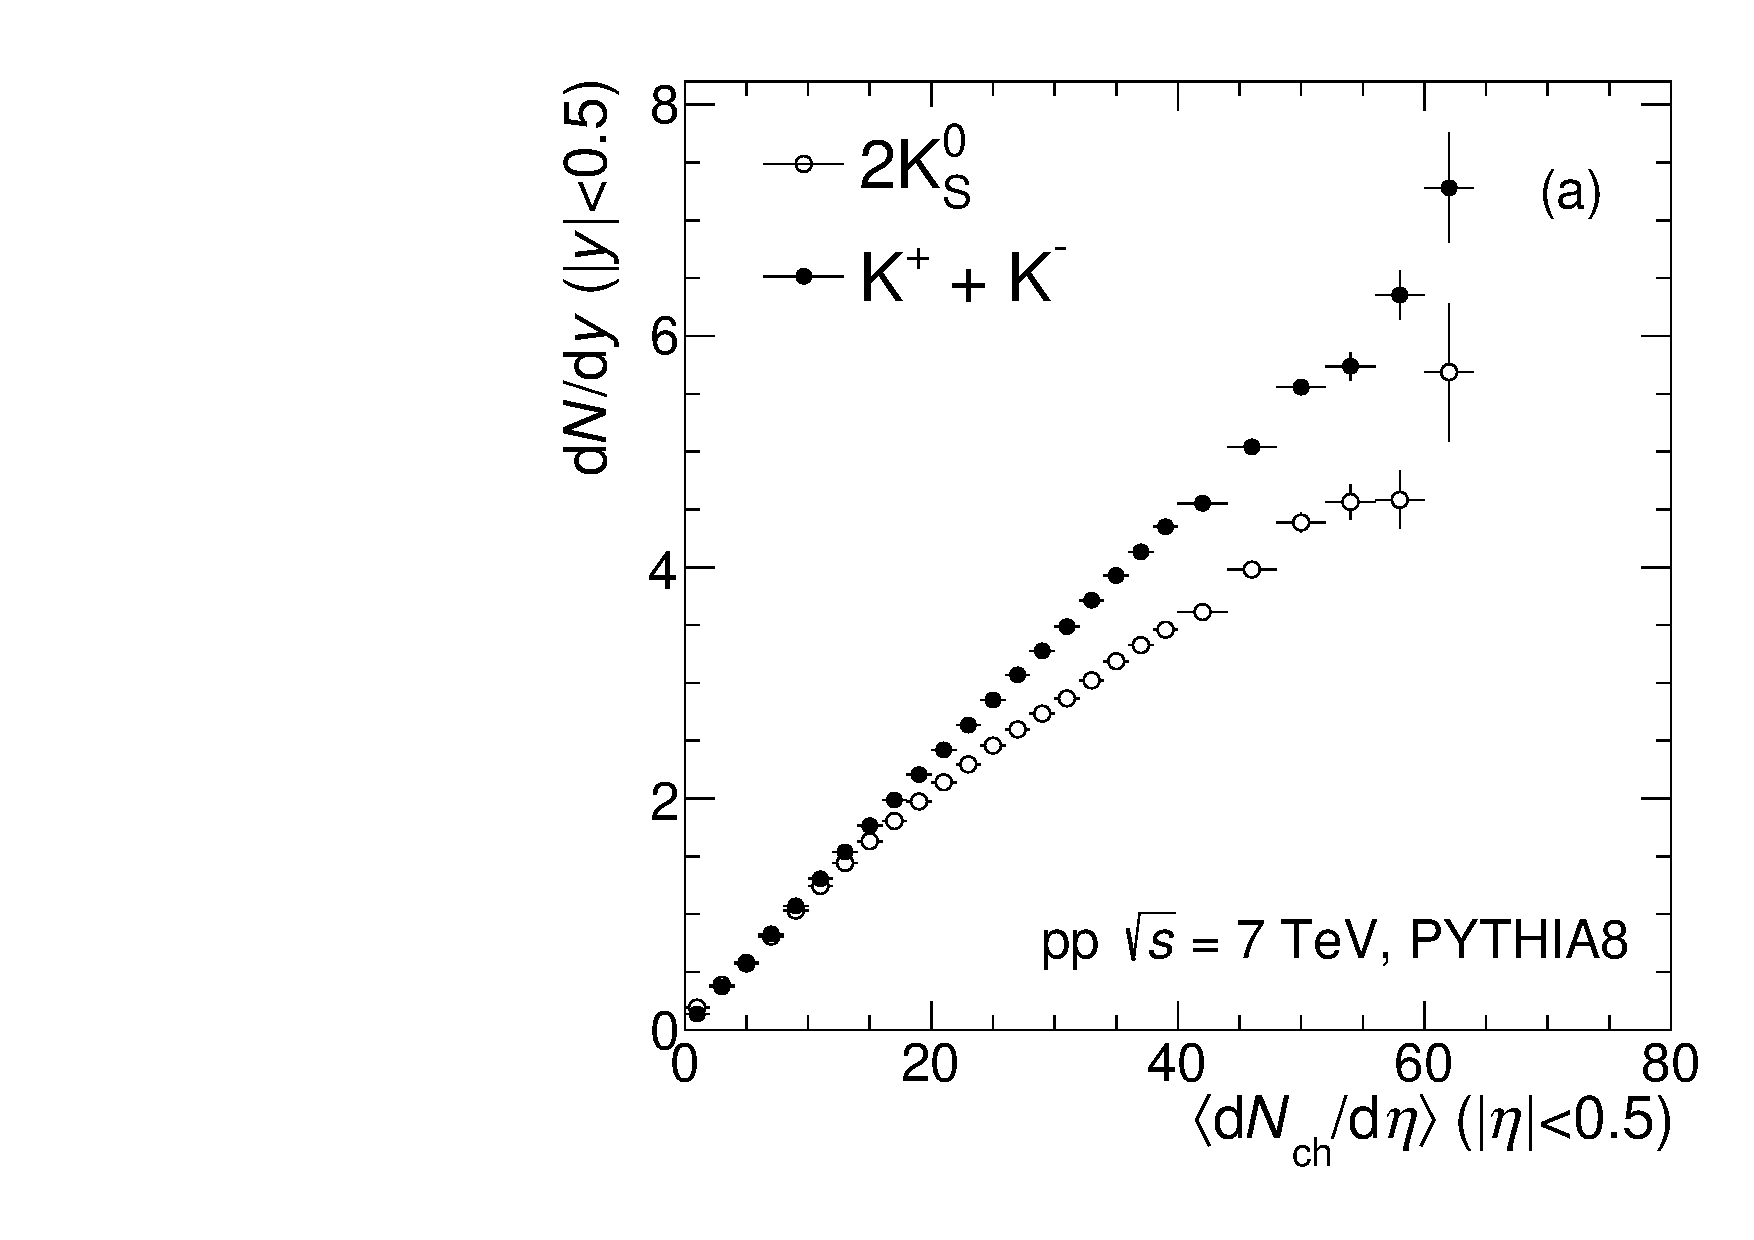
\includegraphics[width=0.475\textwidth]{figures/KchVsK0-MidMult.pdf}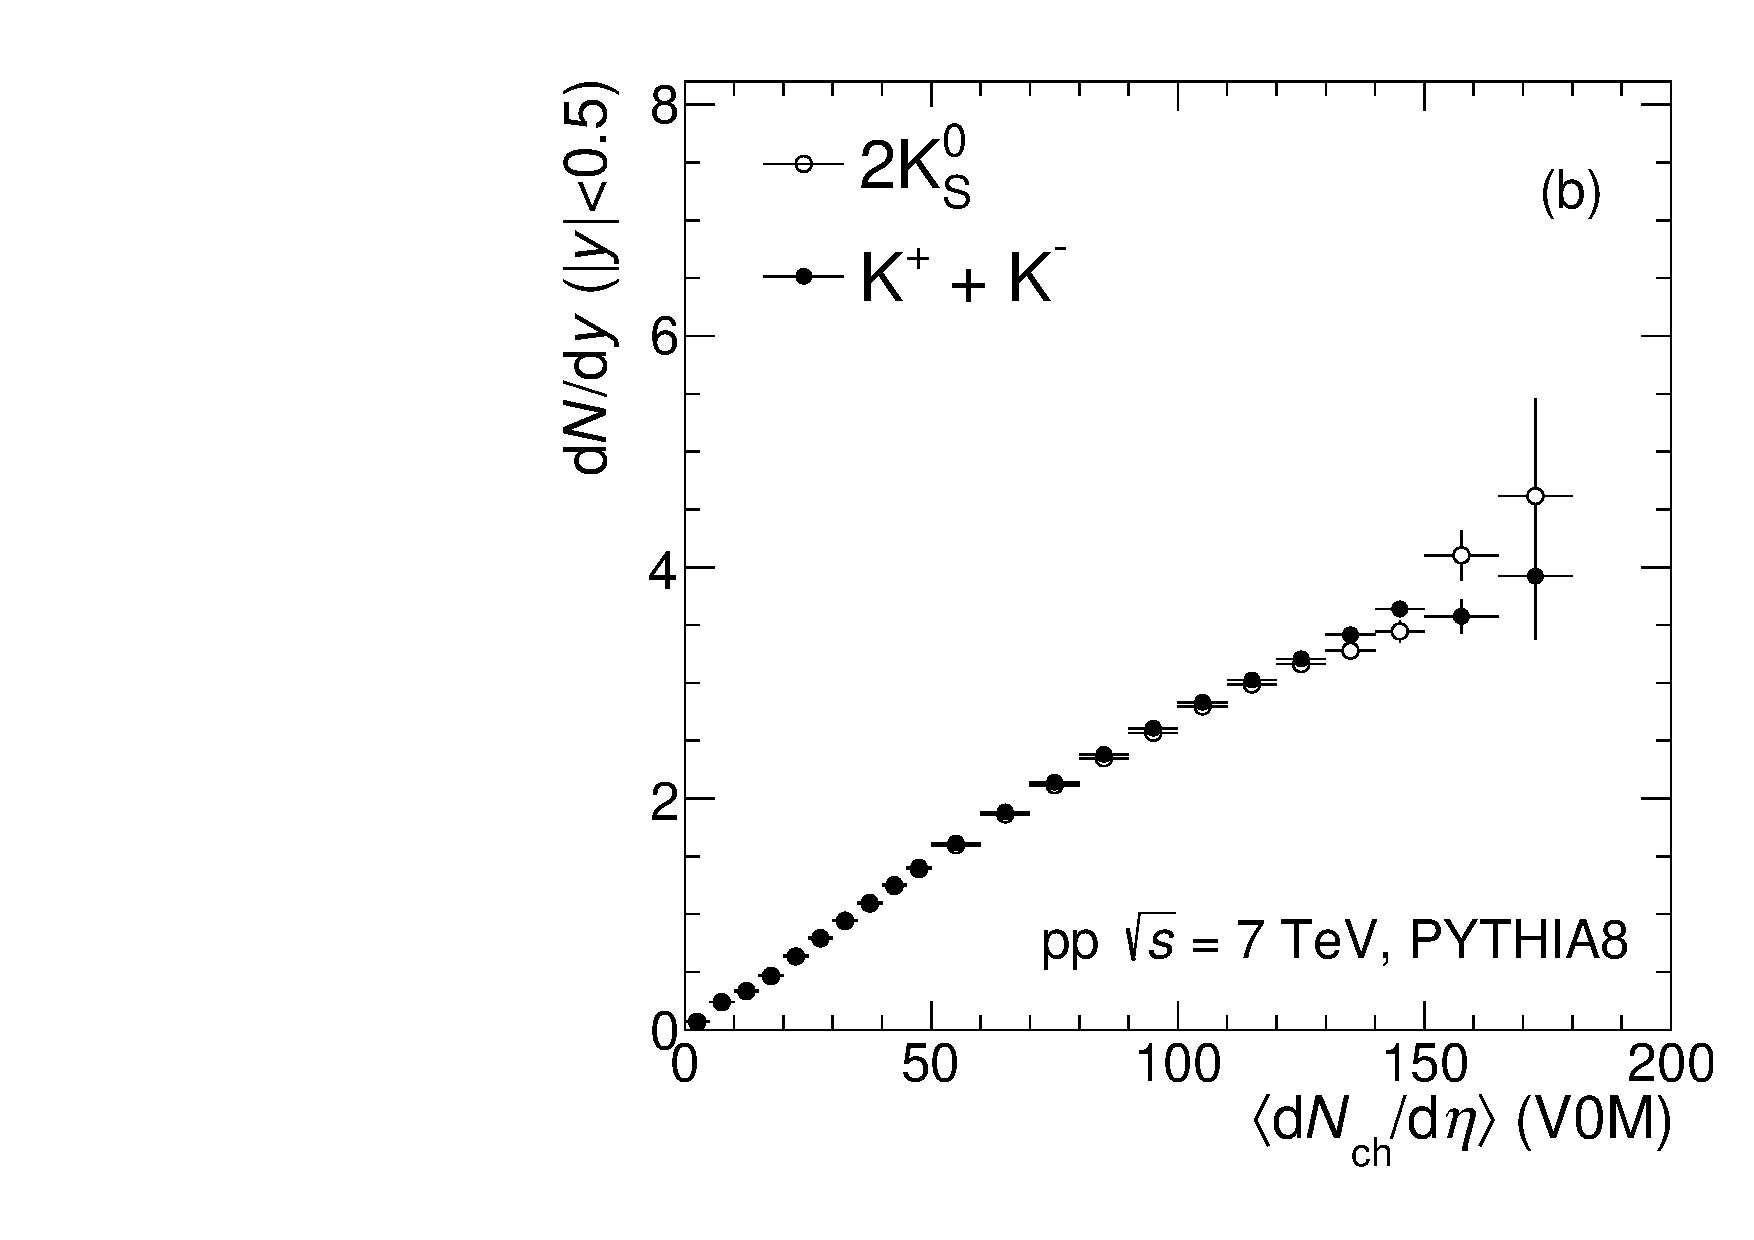
\includegraphics[width=0.475\textwidth]{figures/KchVsK0-V0MMult.pdf}}
%    \end{flushleft}
    \caption{Multiplicity dependence of charged and neutral kaon yields obtained using (a) mid-pseudorapidity charged particle multiplicities ($|\eta|<0.5$) and (b) the charged particle multiplicities within
    the pseudorapidity range corresponding to the V0A and V0C detectors (denoted by V0M, corresponding to $-3.7<\eta<-1.7$ and $2.8<\eta<5.1$) in PYTHIA8 simulations of inelastic pp 
    collisions at \seven.}
    \label{fig:selectionbiases}
\end{figure*}  


This discrepancy for charged and neutral kaons is understood to be a consequence of performing selections on charged-particle multiplicities whose 
probability distributions exhibit a rapid decrease and have low 
average values. Under such circumstances, any multiplicity selections are likely to isolate fluctuations of charged-particle yields in the reference region of 
phase space rather than uniformly affecting all particle species regardless of their charge. In the particular case of \kapm\ and \kzero\ production rates, residual 
differences in these kaon yields still arise from resonance decay products, given that $\phi$ mesons decay preferentially into charged kaons. 
However, Monte Carlo studies show that these different feed-down contributions introduce differences in \kapm\ and \kzero\ yields of no more than 1-2\%, further corroborating 
the need to take into account the much larger selection bias effects shown in Fig.~\ref{fig:selectionbiases}. 

However, while multiplicity selections performed in different phase space regions will avoid selection biases, they are also naturally susceptible to the mid- to 
forward/backward pseudorapidity multiplicity correlation, which for small systems is not as strong as for nuclear collisions~\cite{PhysRevC.91.064905}. 
This has the 
consequence that the reach in midrapidity charged-particle densities is restricted in comparison to same-phase-space selections: when selecting high charged-particle
multiplicities in forward/backward pseudorapidity detectors, midrapidity $\langle {\rm d }N_{\rm ch}/{\rm d }\eta \rangle$ will eventually saturate, while it will still increase 
if event selection is performed with detectors at midrapidity. 
Furthermore, the V0 scintillators
that are used in this work for forward/backward charged-particle detection and event classification introduce an imperfect detector response into the analysis. In order
to minimize potential biases coming from these factors, 
all observables are studied as a function of charged-particle density at midrapidity $\langle$\dNdeta$\rangle$. By doing so, both \dNdeta\ and 
the variables under study are similarly folded with mid- to forward/backward pseudorapidity multiplicity correlations as well as the detector response within a given event class. 
This allows comparing results from this study with predictions from models by performing selections on charged-particle production in 
the acceptance of the V0 and it has been verified that any residual effect because of the finite detector resolution is negligible. 
